\chapter[Studies on Password Selection and Personality Traits]{Understanding Password Selection Through the Lens of Personality Traits}\label{chap:pws_and_personality}

first mentioned in \cite{Weirich2001PrettyGoodPersuasion} that personality could make a difference

more related work: Groß \etal \cite{Gross2016CognitiveDepletion}

\section{Introduction}

% SET THE SCENE

% 1. Passwords are a burden for all of us, and it is getting worse. Users have a portfolio, but what is it made of and why?
As passwords remain the main authentication method on the web, users face an ever increasing challenge to select and maintain passwords. Users' strategies to mitigate this burden are often predictable, such that they use easily guessable passwords and re-use them on more than one service. If required to change a specific password, e.g. after a database breach occurred, users often simply pick another from their own password portfolio \cite{Bonneau2015ImperfectAuthentication, Florencio2014PasswordPortfoliosFiniteUser, Stobert2014PasswordLifeCycle}. How users decide among alternative passwords is a highly individual process, and it is an open question how individual predisposition of the psyche influences the decision making in these situations.
%Although the motivation for acting this way is well understood, we do not know how much of this kind of predictable behavior can be explained by looking at the user's psyche.  
%Although we have indication that passwords are maintained for a long time \cite{VonZezschwitz2013SurvivalShortest}, we know little about the influencing factors on how the actual portfolio comes to be. 


% 2. demographics and education do not explain everything about privacy attitudes, personality and GDMS are valuable.
Apart from demographic and educational factors that evidently affect password creation and coping strategies \cite{Mazurek2013Measuring}, researchers in usable security and privacy have started considering psychological variables to improve explanations for predictable user behavior. Two prominent examples for such variables are the Big-Five personality traits \cite{Goldberg1990BigFive} and the general decision making style (GDMS) \cite{Scott1995GDMS}. The Big Five model tries to characterize a person's attitudes and behavior with five distinct traits, namely openness, conscientiousness, extraversion, agreeableness and neuroticism. The GDMS model describes how people decide by classifying decision-making into rational, intuitive, dependent, avoidant and spontaneous styles. How users form privacy attitudes has been explored extensively \cite{Acquisti2005PrivacyRationality,Korff2014TooMuchChoice,Spiekermann2001EPrivacyPreferences,Woodruff2014PrivacyFundamentalist}. Egelman and Peer, however, were one of the few who suggested taking the Big-Five traits and decision making style into account to explain the preconditions for privacy attitudes \cite{Egelman2015AverageUser}. They found out that someone's decision making style is more predictive than personality traits regarding general privacy attitudes. %In this paper, we investigate if this is also true for another crucial type of privacy behavior, which is to judge the strength of passwords. 

% 3. creating a password is also a decision making process. 
% 4. password strength perceptions have been explored for average users, but where are the individual differences? 
%    --> why are the individual differences necessary?
%    --> why do we think that the differences could result from personality or decision making style?

Decision-making tasks can also be found in password selection: When a user is required to create a password, he or she can either come up with a new one by combining letters, digits and symbols or pick an old password from his or her personal portfolio that usually consists of around five distinct passwords \cite{Florencio2007LargeScaleStudyPasswordHabits}. In any case, the outcome of this decision-making process depends on evaluating ease of typing, memorability, or the perceived strength. When users judge the strength and memorability of passwords, they do this in predictable ways \cite{Ur2016PerceptionsPassword}. They often base their judgment on the variety of characters forming the password. Although there are indeed certain themes in the way users perceive strength, the perceptions are not shared unanimously among all users. Examining what causes the discrepancies is important to help users better understand password strength and to design usable support systems. We hypothesize that the perception of password strength may be influenced by variables like personality traits or decision making style. 

In this paper, we investigate the associations between the Big-Five personality traits, general decision making style and users' perceptions of password strength. In an online study with 100 participants, we administered psychometric tests and collected subjective strength ratings of diverse passwords. We examined the associations between the psychometrics and password strength ratings. Among our key findings, we observed that respondents with high openness scores were more skeptical than the rest about the strength of passwords shown in the study. Moreover, those who score high on conscientiousness were more likely to compare two given passwords by the variety of characters. Rational decision makers performed significantly worse in identifying the stronger of two given passwords.

\subsection{Research Questions}
We posed the following research questions before we set out to conduct the study.\\
\textbf{RQ1 - Psychological Factors} How much do psychological factors affect the perceived strength of passwords?\\
\textbf{RQ2 - Big-Five vs GDMS} Are the Big-Five traits stronger or weaker predictors for strength perception than other psychological variables?\\
\textbf{RQ3 - Portfolio Factors} Is the personal password portfolio associated with strength perception?

\subsection{Contribution Summary}
% CONTRIBUTION STATEMENT:
Our work is one of the first to specifically investigate the relationship between personality traits, decision-making style and perceived password strength. We contribute evidence for (a) the existence of associations between the openness and consciousness traits and password strength assessment. We show that (b) users who show a rational decision making style perform worse in identifying stronger passwords than those who decide intuitively. Furthermore, we (c) conclude that the Big-Five traits were somewhat more predictive than general decision-making style, but that they should be combined depending on the problem. We also identified that (d) the composition of a personal password is also associated with the perception of other passwords. The contributions can help to inform the design of more usable password policies and real-time feedback, as outlined in Section \ref{sec:implications}.


\section{Background and Related Work}
%We position our work in usable security and privacy, in particular password research. Moreover, we include psychological models to better understand users dealing with passwords. 
In this section we give a brief overview about the characteristics of strong passwords and how users go about creating them. Moreover, we portray projects in usable security and privacy research in which the users' psyche has been the focus. 
% secondary
%premise
%influencing 
%preconditions


\subsection{Password Strength Metrics}
%First of all, strong passwords are desirable to protect personal information, 
%TODO motivation: Why do we need strong passwords? Do they achieve anything?
%TODO wir brauchen noch den Hinweis, dass z.B. Substitutionen oder erratbare Modifikationen nicht viel bringen. 
%\subsubsection{Metrics}
Finding an objective and reliable measure for the strength of a given password is difficult. The NIST-entropy of a password is a standard and commonly used measure. It reports the degree of randomness of the characters inside a password \cite[ Appendix A therein]{Burr2011NIST}. However, as more advanced threat models emerged, more realistic measures were proposed. In offline-attack scenarios, the entire database containing the passwords as hashes is obtained by the attackers, which happens sporadically even with highly frequented services like LinkedIn \cite{Florencio2007DoStrongWebPasswords,Scott2016ProtectingLinkedIn,Shay2016DesigningPasswordPolicies}. This means attackers can try millions of times to guess passwords and their efforts are only limited by time and computing power. Multiple researchers proposed that the number of guesses required to crack a password is often a more accurate metric for strength \cite{Kelley20012GuessAgain, Shay2016DesigningPasswordPolicies, Weir2010MetricsPolicies}. Carnegie Mellon University has established a Password Guessing Service (PGS) that allows uploading a list of passwords and receive success rates from various cracking approaches \cite{Ur2015MeasuringRealWorldAccuracies}. To use the service, however, the passwords need to be collected and uploaded in clear-text. This is not always possible in password studies, mostly for ethical reasons. There are other means to estimate the required number of guessing attempts. For example, the zxcvbn algorithm shows high accuracy up to one million guesses, which is a realistic cut-off threshold for online attacks \cite{Wheeler2016zxcvbn}. It can be implemented as a lightweight script and is easy to include in pro-active password checks.

%Moreover, since sophisticated attacks often start with checking for already known passwords, obtaining clear text data goes along with attackers improving their approach. A password that was strong before can quickly become very weak.  
%TODO eventuell noch das DING WANG paper und oder das Neural Network Ding vom Melicher zitieren.

\subsection{Human Factors in Password Strength}
Leaked data from real-world accounts has repeatedly shown that user selected passwords are often predictable \cite{Bonneau2012ScienceOfGuessing}. Given the freedom to select any password, many people opt for simple, short, memorable words or numbers that are easy to type. Because such passwords are vulnerable to informed guessing attacks, service providers try to prevent them by introducing a set of requirements to reduce the risk of account hijacking. However, such composition policies are not implemented identically on all web services \cite{Wang2015EmperorsPolicies}. Often, when users create an account, they re-use a password from elsewhere \cite{Das2014TangledWeb}, which is sometimes prevented if policies differ in requirements. Users then often modify the password until the requirements are met \cite{Inglesant2010TrueCostOfUnusablePolicies,Komanduri2011OfPasswordsAndPeople}. The resulting passwords do not necessarily gain strength, if they are only appended by digits or symbols at predictable positions \cite{Weir2010MetricsPolicies}. Thus, balancing the demands in terms of usability and security of a password policy is challenging and has been under constant research in the past few years \cite{Melicher2016UsabilityMobileTextPasswords,
	Shay2016DesigningPasswordPolicies, 
	Shay2014CanLongPasswordsBeSecureAndUsable,
	Wang2015EmperorsPolicies}. One important aspect of password policies that possibly affects how users evaluate password strength is their educational effect. Users are often exposed to requirements that do not necessarily lead to stronger passwords. The length of the password is often more crucial for the strength than character diversity. For instance, when policies require three different character classes with minimum length twelve (3class12), user-selected passwords are often more guessable than those created with a simple length requirement of 16 characters (basic16) \cite{Shay2014CanLongPasswordsBeSecureAndUsable}. At the same time, users are being told that character variety is necessary to form strong passwords \cite{Ur2012HowDoesYourPasswordMeasureUp}. The long-term consequences are that users sometimes have a suboptimal perception of the factors that add to the objectively measurable strength of a password \cite{Ur2016PerceptionsPassword}. %To this point, psychological factors affecting the susceptibility to educational effects of password policies are underexplored, which we try to   
%HH: Das könnte man mit einem Beispiel unterstützen. Ich denke, das klassische Beispiel ist, dass die Länge wichtiger ist als ob eine Zahl vorkommt.




%\subsection{Studies of Personality in Cyber Security}
\subsection{What Else Influences Password Choice?}
%TODO subconscious? 
%not exhaustive
Beside the constraints dictated by composition policies, many users have developed coping strategies for handling authentication tasks \cite{Stobert2014PasswordLifeCycle}. For example, the value of an account is decisive whether users pick a strong or weak password from their portfolio. Stobert and Biddle argue that this process is deliberate and even IT experts are prone to choose weak passwords for accounts that they do not deem worthy to protect  \cite{Stobert2015ExpertPassword}. Flor\^{e}ncio and Herley argue that this behavior is rational from an economics and efficiency perspective \cite{Florencio2014PasswordPortfoliosFiniteUser}. Still, if users receive security advice by trusted peers, they might reconsider behaviors like password re-use \cite{Das2014EffectSocialInfluenceSecuritySensitivity}.

However, apart from such conscious behavior, there may be other preconditions that make some users pick stronger passwords than others. In a large field study, Mazurek et al. found that computer science and engineering students created passwords that were less guessable than those from business or politics students \cite{Mazurek2013Measuring}. Beyond demographic background, context factors like the emotional state during password selection have also been investigated. Gulenko examined the effect of presenting positive textual messages and icons during password selection and found benefits for the adoption of passphrases \cite{Gulenko2014PasswordsEmotion}. In contrast, putting users in a state of cognitive distress or depletion made participants choose weaker passwords in a large lab study \cite{Gross2016EffectCognitiveEffort}. Social pressure as another type of psychological leverage was investigated by Egelman \etal \cite{Egelman2013DoesMyPasswordGoUpToEleven}. While they argue that account value plays a superior role for the effectiveness of password meters, others have shown that the design of a password meter does have a measurable impact on the effort users put into creating a password \cite{Ur2012HowDoesYourPasswordMeasureUp}. Moreover, password creation can be subtly influenced by suggesting strong passwords at the opportune moment. In a controlled online study, participants created stronger passwords if a longer password was shown beneath the password input field \cite{Seitz2016SuggestionsDecoy}. 
%It was also shown that nudging is effective to make users try and increase password strength. Presentation effects of the nudges can play a role. For example, the design of a password meter can impact how much effort users put into the creation of the password \cite{Ur2012HowDoesYourPasswordMeasureUp}. If shown suggestions, participants in a controlled online study created stronger passwords depending on the kind and number of suggestions \cite{Seitz2016SuggestionsDecoy}. Another intrinsic factor is the degree and type of exposure to social influence in the form of stories or advice. Das et al. showed that such advice affects the intrinsic motivation of acting more secure on the web \cite{Das2014EffectSocialInfluenceSecuritySensitivity}. 

In summary, the literature shows that password selection depends on context factors beyond education and experience. 
\subsection{Personality Factors in Cyber Security}
In our work, we are interested in context factors of password strength originating from psychological variables like personality. One of the most commonly used models to characterize personality are the Big-Five traits, also known as the five-factor model. Costa and McCrae \cite{Costa1992NEO} refer to the personality traits as \textit{openness to experience}, \textit{conscientiousness}, \textit{extraversion}, \textit{agreeableness}, and \textit{neuroticism} (OCEAN). The traits can be described with these exemplary adjectives \cite{McCrae1987ValidationFFM}:\\
\textbf{Openness:} imaginative, creative, curious, independent, liberal\\
\textbf{Conscientiousness:} careful, reliable, ambitious, scrupulous, neat, punctual\\
\textbf{Extraversion:} sociable, talkative, passionate, warm\\
\textbf{Agreeableness:} selfless, helpful, forgiving, cheerful, humble\\
\textbf{Neuroticism:} worrying, emotional, insecure, impatient, vulnerable, subjective

Most frequently, the influence of these personality traits have been explored for privacy-concerns, where the openness trait was associated with privacy attitudes \cite{Egelman2015PredictingAttitudes,Minkus2014PersonalizationPrivacy}. Other inquiries have shown that personality traits like neuroticism \cite{Halevi2013PilotStudyPersonality} or openness \cite{Uebelacker2014SocialEngineering} might be associated with the response to phishing attacks. The likelihood of employees adhering to security policies is potentially influenced by the manifestation of agreeableness and conscientiousness \cite{Shropshire2006PersonalityITSec,Shropshire2015}. These investigations show that personality trait models are a considerable factor in security and privacy. Yet, our understanding of the influence of personality on password perception and consequently password selection is still low. Our work tries to improve our understanding about the origin of the differences in users' judgments of password strength. 
%is linked to these aspects, because passwords protect privacy of users and sensitive data of companies. %However, how password behaviors are formed and how much of the  is explained by psychological factors is still underexplored

%%%%%%%%%%%%%%%%%%%%%%%%%%%%%%%%%%%%%%%%%%%
%%%%
%%%%
%%%%			STUDY 
%%%%
%%%%
%%%%%%%%%%%%%%%%%%%%%%%%%%%%%%%%%%%%%%%%%%%
\section{Study 1: Strength Perceptions and Personality}
With an observational online study, we explored the associations between psychological variables and password strength perception. We regard the perception of strength as necessary step before looking at actual behavior, which is more difficult to observe. Hence, we tried to find associations between subjective password strength ratings and scores on well-established psychometric scales. Before we ran the study, we pre-registered the experiment with the open-science framework (OSF)\footnote{\url{https://osf.io/}, last accessed 11.09.2016} and conducted all analyses as predicted to mitigate confirmation bias. Since we consider our research efforts mostly exploratory, we approached the study without specific hypotheses regarding the influence of certain personality traits or decision making styles on the perception of password strength.

\subsection{Structure}
% DEMOGRAPHICS
The study was divided into six parts of which two were standard psychometric tests. After a brief introduction where the participants were informed about the background of the study, they answered basic demographic questions about gender, age, educational and professional background. %This information is important for the ratings on the password scales, because advanced knowledge in IT(-security) may lead to a different rating than the general audience. 

% META STATISTICS / CREATION
The second part was about collecting characteristics about the passwords that our participants used on real online accounts. Here, we asked about typical password attributes, like LUDS (lower-, uppercase, digits, symbols), length and the inclusion of dictionary words. The collection of such password descriptions is an ethically reasonable way to study actual behavior that does not directly involve creating and disclosing an entire password \cite{VonZezschwitz2013SurvivalShortest}. Participants could select from a list of accounts that they used on a regular basis, e.g. Facebook, YouTube, Netflix, Google. If they did not have any of the selectable accounts they could provide another. The description of a participant's password is called \textit{meta password} in the remainder of the paper. 
%TODO entscheiden ob das reinkommt Additionally we had them create a password which they would rate as sufficient to protect such an online account and that is memorable. We asked not to enter a password that they were currently using. At the end of the study, we again inquired after the fictional password to measure short-term memorability. 
\begin{table}[htbp]
  \centering
  \caption{Set of passwords that we divided into different length and strength categories (as measured with zxcvbn). Features: U = uppercase, D = digits, S = symbols}
 % \small
    \begin{tabular}{lllcccr}
    \multicolumn{1}{c}{\multirow{2}[1]{*}{Password}} & \multicolumn{2}{c}{Categories} & \multicolumn{3}{c}{\multirow{2}[1]{*}{Features}} & \multicolumn{1}{c}{guesses} \\
      & Length & Strength & \multicolumn{3}{c}{} & \multicolumn{1}{c}{(log10)} \\
    \midrule
    hagrqqqqthhbbe & Long & Strong & \multicolumn{3}{c}{-} & 12.48 \\
    etuhcarap & Short & Weak & \multicolumn{3}{c}{-} & 4 \\
    AbWxCdYz & Short & Medium & \multicolumn{3}{c}{U} & 8 \\
    1qaz2wsx3edc & Long & Weak & \multicolumn{3}{c}{D} & 3 \\
    a6a4ba8a & Short & Medium & \multicolumn{3}{c}{D} & 8 \\
    ieatkale88 & Short & Medium & \multicolumn{3}{c}{D} & 10 \\
    thedzfhg123 & Short & Medium & \multicolumn{3}{c}{D} & 10 \\
    11Nd1sPPut8ble99 & Long & Strong & \multicolumn{3}{c}{U,D} & 16 \\
    bicycles-peaches-cold & Long & Strong & \multicolumn{3}{c}{S} & 13.69 \\
    AatIcs,ijayl-t & Long & Strong & \multicolumn{3}{c}{U,S} & 13.95 \\
    p@ssw0rd & Short & Weak & \multicolumn{3}{c}{D,S} & 0.95 \\
    ocean4 Size !beer Car & Long & Strong & \multicolumn{3}{c}{U,D,S} & 20.39 \\
    F@m1Ly07\% & Short & Medium & \multicolumn{3}{c}{U,D,S} & 6.88 \\
    \bottomrule
    \end{tabular}%

  \label{tab:password-list}%
  
\end{table}%

%  RATING
In the third part of the study, the \textit{rating part}, the participants assessed the strength of one password at a time in random order. The passwords had to be rated on 7-point scales ranging from \textit{1 = very weak} to \textit{7 = very strong}. We picked a set that was comparable to related work \cite{Ur2016PerceptionsPassword} and that we carefully designed around certain attributes. Table \ref{tab:password-list} shows the selected set of passwords and their features. The ``length'' category distinguishes between short passwords with nine characters or less and long passwords with ten characters or more. The distinction is inspired by real-world policies that usually require nine or more characters \cite{Wang2015EmperorsPolicies}. Other passwords are usually ``below that bar'' and can thus be considered too short. The ``strength'' category groups passwords on three levels by their objective guessability as measured by zxcvbn. Weak passwords require less than $10^{6}$ guessing attempts, strong passwords at least $10^{12}$ guesses, and medium passwords anything in between. This classification is in concordance with related work \cite{Florencio2014AdministratorsGuide, Wheeler2016zxcvbn} . To fully counterbalance all category combinations, one would require 120 items, which we could not implement for the sake of brevity. Hence, we kept the number of items small to mitigate fatigue during the study sessions. In the chosen set of 13 passwords, there were at least three items for each distinct category, i.e. three short, long, weak and strong passwords, and at least three passwords containing at least one of LUDS features (lowercase, uppercase, digits and symbols)

% COMPARISON
Following a similar procedure as Ur et al. \cite{Ur2016PerceptionsPassword}, participants moved on to compare the strength of passwords pairs (\textit{comparsion part}). The 7-point scale ranged from ``<left password> is much stronger'' to ``<right password> is much stronger''. The pairs were constructed such that the passwords differed, e.g., in the existence and positions of digits and uppercase letters. Figure \ref{fig:comparisontask} illustrates our scoring schema. 

\begin{figure}
	\centering
	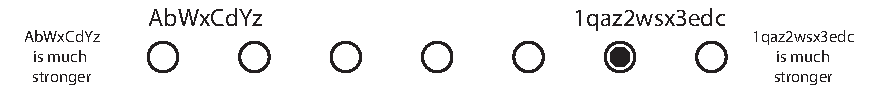
\includegraphics[width=\linewidth]{figures/comparisontask}
	\caption{\label{fig:comparisontask} Simplified item of the comparison task. The passwords differ in length, strength, and the usage of uppercase letters and digits. Here would have scored the importance of length and digits with +2 while the importance of strength and uppercase letters was scored with -2.}
\end{figure}

If the passwords measurably differ in strength as in Figure \ref{fig:comparisontask}, the ratings show if the participants' perceptions match reality. In total, ten comparisons had to be made in random order, in which we permuted the combinations. For this task, we also added an attention check where the passwords on both sides of the scale matched, allowing us to exclude responses where the answer differed from ``both passwords are equally strong''. 

Next, we requested self-assessment about security-related behavior using the Security Behavior Intentions Scale (SeBIS) \cite{Egelman2015SeBIS}. This scale comprises the dimensions \textit{securement}, \textit{passwords}, \textit{awareness}, and \textit{updating}. For each dimension, a score is calculated with four items totaling up to 16 additional items in our study. However, in discussions after the experiment we received hints that it would have been better to include a gap of a couple of days before collecting the SeBIS data to ensure its validity. Since we failed to take this into account beforehand, we do not report the results further, but it is important to mention that the questionnaire included 16 additional items. 
%The items are phrased as statements to which respondents can indicate how often they show a certain type of security-related behavior. The scale ranges from \textit{1 = never} to \textit{5 = always}. The \textit{password} dimension measures general attitude towards passwords, which we can utilize to inform our interpretation later.

The study concluded with two psychometric tests. In the \textit{Big-Five part}, we utilized a set of 50-items from the International Personality Item Pool (IPIP), which is a representation of Costa and McCrae's NEO-PI-R domains \citep{Costa1992NEO}\footnote{All items of the personality test can be found here: \url{http://ipip.ori.org/newNEODomainsKey.htm}, psychometric properties: \url{http://ipip.ori.org/newNEO_DomainsTable.htm}}. In this personality test, participants rate how accurately a certain statement portraying a certain personality characteristic describes themselves. Each item is a 5-point scale with the labels \textit{very inaccurate, moderately inaccurate, neither accurate nor inaccurate, moderately accurate, very accurate}. Every personality trait is tested with five positively and five negatively keyed items. It was shown that the 50-item version of the test shows high correlation with more exhaustive tests ($r > 0.75$ in all dimensions) and is thus a sufficiently reliable test. We randomized the order of the items.

Egelman and Peer found that the general decision making style had higher predictive power than the Big-Five traits for privacy-related behavior \cite{Egelman2015AverageUser}. Thus, we wanted to test the feasibility of both psychometric tests and finished the study with the \textit{GDMS part}. This scale uses 25 positively keyed items to measure the five decision-making styles \textit{rational}, \textit{intuitive}, \textit{dependent}, \textit{avoidant} and \textit{spontaneous}. 

\subsection{Quantitative Analysis}
We used a set of statistical tests to explore the relationship between the scores psychometric scales and password strength perception. Since at least three passwords showed a certain characteristic, e.g. uppercase letters, we averaged the ratings for them accordingly. Moreover, in the psychometric tests we accounted for negatively keyed items, i.e. those items that were phrased with negations like \textit{``I don't talk a lot''}. We inverted the ratings where necessary and afterwards calculated the sum of agreement for each dimension. 

We use linear regression with subjective password strength assessments as dependent variables. We calculate one score per participant and password category by averaging the corresponding ratings. Psychometric test results on sub-scales served as independent variables. We always control the regression models for gender, technical background and education level to prevent misinterpreting the effects. Education was coded as ordinal variable from 1 (grammar school) to 7 (professional degree like PhD, MD, JD). Before performing regressions, we check for collinearity using variance inflation factors (VIF) and only retain factors with VIFs close to 1 \cite[p. 217]{Weisberg2005applied}. Also, because of the exploratory nature, we can use step-wise regression methods to build the models. To mitigate type-II errors herein, we use a backward approach \cite[p. 161]{Field2005DiscoveringStatistics} and exclude factors that do not improve the model significantly. Finally, we perform Durbin-Watson tests to rule auto-correlation effects (target value $d=2$). While p-values do not add much to the interpretability of the findings, we report them for the sake of completeness.  
%TODO Quelle!
%Our level for statistical significance is $\alpha = 0.05$, unless Bonferroni correction requires a lower value. 

When we report the results of linear regression models, we only do so for the models with the highest adjusted $R^2$ value, i.e. the model where the number of predictors leads to the best model-fit explaining the variance in the dependent variable. The values in Tables \ref{tbl:personalpw_regression} through \ref{tab:Comparison-Regression} are the \textbf{standardized beta} correlations, i.e. they are unit-less and lie between -1 and +1. 

\subsection{Qualitative Analysis}
To better understand the reasoning behind the ratings and comparisons, we also inquired how the respondents approached the rating task. They could enter free-text answers after all ratings were done. The answers were then coded independently by two members of the team. The first coding step was to find categories and propose the code book. Afterwards, the proposed codes were handed over to the second coder, who sorted answers into the categories and amended new ones where necessary. Interrater agreement between the two coders was satisfactory (78\%, Krippendorff's $\alpha = 0.55$) and the final the code book could be created after discussing the discrepancies. We report how many participants mentioned a particular theme in their response regarding their rating strategies.


\subsection{Recruitment}
We utilized the online research platform Prolific\footnote{\url{https://prolific.ac}, accessed 01.09.2016} to administer our survey. Participants received \$2.65 upon successful completion, which took 20 minutes in average. This compensation level is suggested as part of the ethical reward guidelines on the platform. Only an English-speaking audience was eligible to participate. From the 178 people who started the survey, 104 finished it. To prevent low quality answers, we introduced an attention check during the comparison part of the experiment.  

%In the first phase of the study, the participants were asked to imagine their email provider required them to create a new password and they could not select their current one. This measurement was taken early to prevent bias from showing different types of passwords. The answers were collected in plain text. We proceeded to have the users choose the type of account that they would be willing to secure with their selected password in the real world. This would indicate the effort and the value of their selection.


\subsection{Ethical Considerations}
There is no institutional review board for this kind of studies at our institution. However, we designed the questionnaire to respect the participants' privacy and did our best to minimize the level of disclosure of sensitive data. The metrics we collected to characterize the participants' passwords are most likely insufficient to reconstruct the passwords in a straightforward way and can thus be considered ethically acceptable. 


\subsection{Limitations}
%It is good to discuss the limitations before the results. Thus, the reader can bear them in mind when they are reading on. 

Like most studies involving personality assessment, the result is only a rough model of a person's personality and does not include all facets. We chose a test with 50 items to assess the Big-Five traits. While such psychometric tests exist with item counts between 10 \cite{Gosling2003TIPI} and 240 items \cite{Costa1992NEO}, the 50-item version has high internal reliability and does not fatigue the respondents as much as more exhaustive tests. Additionally, with a sample size of 100 participants, power-analysis tells us, that only strong and medium interactions are likely to be found for with our regression models (cf. \cite{Shevlin1998SampleSize} or \cite[p. 223]{Field2005DiscoveringStatistics}). At this stage of the exploration, however, this is what we aimed for. If we do find effects with such a small sample, then they must be large enough to justify follow-up investigations with larger samples. 

Furthermore, the methodology relies on self-assessment and honest answers, which are difficult to control. We introduced an attention check to mitigate the problem, by asking people to compare two identical passwords. For the meta-password, we do not know whether it was created on a mobile or desktop device. Passwords created on mobiles are usually less complex than those created on desktops \cite{Melicher2016UsabilityMobileTextPasswords, VonZezschwitz2014HoneyIShrunkTheKeys}. 

We also have to be careful not to over-generalize the results due to our use of crowd-sourced study participation. The responses may not be representative for a larger population, e.g. because the sample stems from a technically savvy audience. Users registering for tools like Prolific or Amazon Mechanical Turk may also have stronger financial motivation to do so than the rest of the population \cite{Ross2010WhoAreTurkers}. 

Finally, the study set-up and procedure may also influence the interpretability of the outcome. We decided not to randomize the order of the question blocks to maintain full control over the general procedure. When we measure dependent variables, the order of questions is still randomized in the question groups. This way, the potential fatigue effects are the same for all participants at the different stages, while the important questions are in random order. Moreover, the items for password pairs were not fully counterbalanced on all levels to prevent fatigue when answering the entire questionnaire. A more exhaustive set of tested passwords would increase the generalizability. 

%we need to be aware that a more faceted personality profile may reveal larger differences. 
%TODO viele antworten deuteten darauf hin, dass englisch nicht in die muttersprache ist. 
%TODO meta password characteristics are not an accurate proxy for password strength, as depicted in the background section. 
%Our proxy for password strength is the result of the zxcvbn estimator algorithm \cite{Wheeler2016zxcvbn}. While it can estimate the strength of passwords in attack scenarios up to one million guesses, its estimates become more fuzzy above this threshold. However, for the purpose of the study, the estimate was considered good enough as it still highly correlates with the estimates of more sophisticated tools like the password guessing service (PGS) \cite{Ur2015MeasuringRealWorldAccuracies}. 
%\begin{itemize}
%\item we might measure intelligence
%\item self-reporting might not be accurate
%\end{itemize}


%As we collected plain text passwords that could -- in theory -- be linked backed to an individual, we took special care to point out that participants should not enter their actual password, but to think of a new one. The additional meta characteristics are most likely insufficient to reconstruct a participant's actual password. 

\begin{figure}
	\centering
	\includegraphics[width=\linewidth]{figures/MetaPW-Violinplot}
	\caption{\label{fig:MetaPW-ViolinPlot} Violin plot of strength ratings, grouped by the number of uppercase letters in the participants' meta password. The plot gets broader, the more respondents scored in the particular range. The plot shows a negative association between overall password strength and uppercase letters in the meta password.}
\end{figure}



%%%%%%%%%%%%%%%%%%%%%%%%%%%%%%%%%%%%%%%%%%%
%%%%
%%%%
%%%%			RESULTS 
%%%%
%%%%
%%%%%%%%%%%%%%%%%%%%%%%%%%%%%%%%%%%%%%%%%%%
\subsection{Results}
In this section, we first describe the participants and meta password characteristics before we proceed to the regression analyses. The final part of this section shows qualitative findings and a brief synthesis of the results. 

\subsubsection{Participants}
We collected 104 complete samples. We had to remove three samples from respondents who failed the attention check. Another response was removed because all responses on point scales were answered with the same value. This procedure is proposed by the IPIP project \footnote{\url{http://ipip.ori.org/newValidity.htm} accessed 02.09.2016}. The resulting total N = 100 was divided into 42 female and 58 male participants. Their average age was 28 years ($Standard Deviation~(SD) = 9,~Minimum = 16,~Maximum = 61,~Median~(Md) = 26$). 44 responses came from students. The education level was high with 59 participants reportedly having a bachelor's (44) or master's (15) degree. 29 participants claimed to have a computer science or IT-related background. In summary, our sample stems from a young, educated and fairly technically savvy population. This convenience sample is not ideal, but we hope to deal with this skew by including demographics as predictors in the regression models.

\subsubsection{Strength Categories and Meta Passwords}
On average, the respondents correctly identified weak, medium and strong passwords in the rating task, i.e. their perception matched reality. The average scores were $M=3.60~(SD=1.07)$ for weak, $M=4.25~(SD=0.95)$ for medium and $M=4.71~(SD=0.90)$ for strong passwords. A Friedman rank test showed that these ratings differed significantly ($F(2)=59.91,~p < 0.001$). 

The participants' meta password characteristics are important to find out if past actions influence strength ratings. The participants reported to use passwords that were nine characters long ($Md=9,~SD=3$), which is consistent with the finding that most real-world policies require a minimum of eight or nine characters \cite{Wang2015EmperorsPolicies}. The medians for other password characteristics were 1 uppercase letter ($SD=1$), 2 digits ($SD=3$), 0 special characters ($SD=1$) and 1 dictionary word ($SD=1$).

%\subsubsection{Behavior and Strength Rating}
Before we analyzed the influence of personality traits on the ratings, checked associations between meta passwords and password ratings. We performed linear regression analyses as shown in Table \ref{tbl:personalpw_regression}. The regression models reveal that ratings were mostly associated with the length and usage of uppercase letters inside one's own password. Model fit was $R^2_{adj}=0.12$ for overall rating. Particularly in the second row of Table \ref{tbl:personalpw_regression}, we can see that participants, who report to include more uppercase letters in their meta passwords, were more likely to give lower overall strength ratings (cf. Figure \ref{fig:MetaPW-ViolinPlot}). Regarding the comparison task, we found that the meta passwords were only very weakly associated with the outcome (mean $R^2_{adj}=0.03$). Hence, we do not present detailed statistics. 

% Table generated by Excel2LaTeX from sheet 'Correlation Matrix SLUDS'

\begin{table}%[htbp]
  \centering
  \small
  \caption{Regression analysis with participants' proxy password characteristics as independent variables and ratings for password groups. Especially the use of uppercase letters is negatively correlated with the ratings. Numbers in bold indicate statistical significance ($p<0.05$)}
  \resizebox{\linewidth}{!}{
\begin{tabular}{l|r|rr|rrr|rrr}
    \multicolumn{1}{c|}{\multirow{2}[1]{*}{\textbf{Proxy PW Characteristic}}} & \multicolumn{9}{c}{\textbf{Password Ratings}} \\
      & \multicolumn{1}{c|}{Overall} & \multicolumn{1}{l}{Long} & \multicolumn{1}{l|}{Short} & \multicolumn{1}{l}{Weak} & \multicolumn{1}{l}{Medium} & \multicolumn{1}{l|}{Strong} & \multicolumn{1}{l}{Special} & \multicolumn{1}{l}{Digits} & \multicolumn{1}{l}{Uppercase } \\
    \midrule
    \rowcolor[rgb]{ .922,  .945,  .871} Length & -0.13 &   & -0.12 & \textbf{-0.20} &   &   & \textbf{-0.21} &   & -0.13 \\
    \rowcolor[rgb]{ .922,  .945,  .871} Uppercase Letters & \textbf{-0.33} & \textbf{-0.31} & \textbf{-0.26} &   & \textbf{-0.37} & \textbf{-0.25} & -0.18 & \textbf{-0.41} & \textbf{-0.30} \\
    \rowcolor[rgb]{ .922,  .945,  .871} Digits &   &   &   &   &   &   &   &   &  \\
    \rowcolor[rgb]{ .922,  .945,  .871} Symbols &   &   &   &   &   &   &   & 0.12 &  \\
    IT Background &   &   &   & -0.10 &   &   &   &   &  \\
    Education &   &   & 0.11 &   &   & -0.12 &   &   &  \\
    Gender &   &   &   &   &   &   & 0.20 &   & 0.10 \\
    \midrule
    \textbf{F} & \textbf{7.64} & \textbf{10.29} & \textbf{3.74} & \textbf{3.27} & \textbf{15.33} & \textbf{3.89} & \textbf{3.40} & \textbf{9.45} & \textbf{4.13} \\
    \textbf{p} & 0.00 & 0.00 & 0.01 & 0.04 & 0.00 & 0.02 & 0.02 & 0.00 & 0.01 \\
    \textbf{Adj. $R^2$} & \cellcolor[rgb]{ .675,  .831,  .502} 0.12 & \cellcolor[rgb]{ 1,  .922,  .518} 0.09 & \cellcolor[rgb]{ .992,  .812,  .494} 0.08 & \cellcolor[rgb]{ .973,  .412,  .42} 0.04 & \cellcolor[rgb]{ .592,  .804,  .494} 0.13 & \cellcolor[rgb]{ .976,  .545,  .443} 0.06 & \cellcolor[rgb]{ .988,  .702,  .475} 0.07 & \cellcolor[rgb]{ .388,  .745,  .482} 0.15 & \cellcolor[rgb]{ .992,  .922,  .518} 0.09 \\
    \bottomrule
    \bottomrule
    \end{tabular}%
        }
%  \resizebox{\linewidth}{!}
%{
%
%
%}
  
  \label{tbl:personalpw_regression}%
\end{table}%

\begin{table*}%[h!tbp]
  \small
  \centering
  \caption{Regression analysis for password ratings in different categories as dependent variables and psychometrics as independent variables variables. Demographic data serves as control variables. Numbers in bold indicate statistical significance ($p<0.05$). The Big-Five factors had higher predictive value and than the GMDS factors.}
    \resizebox{\linewidth}{!}
{
\begin{tabular}{rl|r|rr|rrr|rrr}
    \multicolumn{2}{l|}{Predictor} & \multicolumn{1}{l|}{Overall} & \multicolumn{1}{l}{Short} & \multicolumn{1}{l|}{Long} & \multicolumn{1}{l}{Weak} & \multicolumn{1}{l}{Medium} & \multicolumn{1}{l|}{Strong} & \multicolumn{1}{l}{Symbols} & \multicolumn{1}{l}{Digits} & \multicolumn{1}{l}{Uppercase} \\
\cmidrule{3-11}    \rowcolor[rgb]{ .718,  .871,  .91} \multicolumn{1}{l}{Big Five} & Neuroticism & \cellcolor[rgb]{ 1,  1,  1}  & \cellcolor[rgb]{ .949,  .91,  .518} 0.15 & \cellcolor[rgb]{ .949,  .91,  .518} 0.15 & \cellcolor[rgb]{ .969,  .914,  .518} 0.14 & \cellcolor[rgb]{ 1,  1,  1}  & \cellcolor[rgb]{ .98,  .627,  .459} -0.15 & \cellcolor[rgb]{ 1,  1,  1}  & \cellcolor[rgb]{ 1,  1,  1}  & \cellcolor[rgb]{ 1,  1,  1}  \\
    \rowcolor[rgb]{ .718,  .871,  .91}   & Openness & \cellcolor[rgb]{ .976,  .518,  .439} \textbf{-0.25} & \cellcolor[rgb]{ .976,  .541,  .443} \textbf{-0.23} & \cellcolor[rgb]{ .98,  .573,  .447} \textbf{-0.2} & \cellcolor[rgb]{ .976,  .498,  .435} \textbf{-0.27} & \cellcolor[rgb]{ .98,  .616,  .459} -0.16 & \cellcolor[rgb]{ .98,  .604,  .455} -0.17 & \cellcolor[rgb]{ .984,  .647,  .463} -0.13 & \cellcolor[rgb]{ .976,  .541,  .443} \textbf{-0.23} & \cellcolor[rgb]{ .984,  .639,  .463} -0.14 \\
    \rowcolor[rgb]{ .718,  .871,  .91}   & Agreeableness & \cellcolor[rgb]{ .898,  .894,  .514} 0.18 & \cellcolor[rgb]{ .949,  .91,  .518} 0.15 & \cellcolor[rgb]{ .898,  .894,  .514} 0.18 & \cellcolor[rgb]{ .898,  .894,  .514} 0.18 & \cellcolor[rgb]{ 1,  1,  1}  & \cellcolor[rgb]{ .969,  .914,  .518} 0.14 & \cellcolor[rgb]{ .984,  .918,  .518} 0.13 & \cellcolor[rgb]{ .996,  .91,  .514} 0.11 & \cellcolor[rgb]{ 1,  1,  1}  \\
    \rowcolor[rgb]{ .988,  .835,  .706} \multicolumn{1}{l}{GDMS} & Rational & \cellcolor[rgb]{ 1,  1,  1}  & \cellcolor[rgb]{ 1,  1,  1}  & \cellcolor[rgb]{ 1,  1,  1}  & \cellcolor[rgb]{ 1,  1,  1}  & \cellcolor[rgb]{ 1,  1,  1}  & \cellcolor[rgb]{ 1,  1,  1}  & \cellcolor[rgb]{ 1,  1,  1}  & \cellcolor[rgb]{ 1,  1,  1}  & \cellcolor[rgb]{ .984,  .918,  .518} 0.13 \\
    \rowcolor[rgb]{ .988,  .835,  .706}   & Intuitive & \cellcolor[rgb]{ 1,  1,  1}  & \cellcolor[rgb]{ 1,  1,  1}  & \cellcolor[rgb]{ 1,  1,  1}  & \cellcolor[rgb]{ 1,  1,  1}  & \cellcolor[rgb]{ 1,  1,  1}  & \cellcolor[rgb]{ 1,  1,  1}  & \cellcolor[rgb]{ 1,  1,  1}  & \cellcolor[rgb]{ 1,  1,  1}  & \cellcolor[rgb]{ .996,  .898,  .51} 0.1 \\
    \rowcolor[rgb]{ .988,  .835,  .706}   & Avoidant & \cellcolor[rgb]{ 1,  1,  1}  & \cellcolor[rgb]{ 1,  1,  1}  & \cellcolor[rgb]{ 1,  1,  1}  & \cellcolor[rgb]{ .984,  .639,  .463} -0.14 & \cellcolor[rgb]{ 1,  1,  1}  & \cellcolor[rgb]{ 1,  1,  1}  & \cellcolor[rgb]{ .984,  .647,  .463} -0.13 & \cellcolor[rgb]{ 1,  1,  1}  & \cellcolor[rgb]{ 1,  1,  1}  \\
    \rowcolor[rgb]{ .988,  .835,  .706}   & Spontaneous & \cellcolor[rgb]{ 1,  1,  1}  & \cellcolor[rgb]{ 1,  1,  1}  & \cellcolor[rgb]{ 1,  1,  1}  & \cellcolor[rgb]{ 1,  1,  1}  & \cellcolor[rgb]{ .984,  .918,  .518} 0.13 & \cellcolor[rgb]{ 1,  1,  1}  & \cellcolor[rgb]{ .949,  .91,  .518} 0.15 & \cellcolor[rgb]{ 1,  1,  1}  & \cellcolor[rgb]{ 1,  1,  1}  \\
      & Education &   & \cellcolor[rgb]{ .914,  .898,  .514} 0.17 &   & \cellcolor[rgb]{ .984,  .918,  .518} 0.13 & \cellcolor[rgb]{ 1,  .922,  .518} 0.12 &   &   & \cellcolor[rgb]{ .933,  .902,  .514} 0.16 &  \\
      & CS Background & \cellcolor[rgb]{ .984,  .647,  .463} -0.13 &   & \cellcolor[rgb]{ .984,  .647,  .463} -0.13 &   & \cellcolor[rgb]{ .98,  .627,  .459} -0.15 & \cellcolor[rgb]{ .984,  .682,  .471} -0.1 &   & \cellcolor[rgb]{ .984,  .682,  .471} -0.1 &  \\
    \midrule
      & F & 4.23 & 2.83 & 3.54 & 3.46 & 1.9 & 2.48 & 1.91 & 2.52 & 1.19 \\
      & df & 3 & 4 & 4 & 5 & 4 & 4 & 4 & 4 & 3 \\
      & p & < 0.01 & < 0.05 & < 0.05 & < 0.01 & > 0.1 & < 0.05 & > 0.1 & < 0.05 & > 0.1 \\
      & R$^2$ & \cellcolor[rgb]{ .761,  .898,  .804} 0.12 & \cellcolor[rgb]{ .788,  .91,  .827} 0.11 & \cellcolor[rgb]{ .733,  .886,  .78} 0.13 & \cellcolor[rgb]{ .675,  .863,  .729} 0.15 & \cellcolor[rgb]{ .906,  .957,  .929} 0.07 & \cellcolor[rgb]{ .82,  .922,  .855} 0.1 & \cellcolor[rgb]{ .906,  .957,  .929} 0.07 & \cellcolor[rgb]{ .82,  .922,  .855} 0.1 & \cellcolor[rgb]{ .988,  .988,  1} 0.04 \\
      & Adjusted R$^2$ & \cellcolor[rgb]{ .706,  .875,  .757} 0.09 & \cellcolor[rgb]{ .776,  .906,  .82} 0.07 & \cellcolor[rgb]{ .706,  .875,  .757} 0.09 & \cellcolor[rgb]{ .635,  .847,  .698} 0.11 & \cellcolor[rgb]{ .882,  .949,  .91} 0.04 & \cellcolor[rgb]{ .812,  .918,  .851} 0.06 & \cellcolor[rgb]{ .918,  .961,  .941} 0.03 & \cellcolor[rgb]{ .812,  .918,  .851} 0.06 & \cellcolor[rgb]{ .988,  .988,  1} 0.01 \\
    \bottomrule
    \bottomrule
    \end{tabular}%
}
  \label{tab:Regression-Rating}%
\end{table*}%

%%%%%%%%%%%%%%%%%%%%%%%%%%
%%% 
%%% 		STRENGTH RATING
%%% 
%%%%%%%%%%%%%%%%%%%%%%%%%%
\subsubsection{Standalone Strength Rating}
Our next step was to analyze associations between personality, respectively decision making style and password perception. After having done all required assumption checks, including internal consistency analysis of the scales ($\alpha_{IPIP}=0.72, \alpha_{GDMS}=0.8$), we built regression models containing the scores on the big-five subscales, the GMDS scores and control variables. The initial model hence included the independent variables \textit{openness, conscientiousness, extraversion, agreeableness, neuroticism}, as well as the \textit{rational, intuitive, dependent, avoidant, spontaneous} decision making scores. We added gender, IT-background and education level as controlling factors. The initial model contained all factors and was refined in a backward stepwise removal approach, leaving only those factors with highest predictive values. 

Table \ref{tab:Regression-Rating} shows the regression results of standalone password ratings. The overall ratings in the first column, which we consider the most important metric, were negatively associated with the \textit{openness} trait ($\beta = -0.25, p < 0.05$) (see also Figure \ref{fig:openness-scatterplot}). In other words, participants with higher openness scores were generally more pessimistic regarding password strength, which was also the case if participants had a technical background, albeit this association was not as strong. Higher agreeableness scores were slightly associated with more optimistic overall password ratings. Interestingly, with conscientiousness and extraversion, two of the big-five factors never played a significant role and thus are omitted in Table \ref{tab:Regression-Rating}.

The decision making style predictors were retained in four of the nine models, but never showed high predictive power. Contrarily, the openness trait was retained in the regression models across the board. For example, especially the weaker passwords receive lower ratings from people with higher openness scores. However, the average adjusted $R^2$ across all categories tells us that the models explain only a rather small portion of the variance in the password ratings ($M=0.06~(SD=0.03)$). 

%The lower half of Table \ref{tab:B5-Regression-Comparison} shows the analysis results for standalone password ratings. One can see that there were no striking associations between predictors and dependent variables. Also, the models with the highest $R^2$ value needed six degrees of freedom on average. This means that no particular decision making style stands out to inform the predictions. The maximum $R^2$ value across the models here is $0.05$, i.e. very low. Thus, decision making style did not explain variances satisfactorily.

\begin{figure}
	\centering
	\includegraphics[width=\linewidth]{figures/Openness-ScatterPlot3}
	\caption{\label{fig:openness-scatterplot} Scatter plot of openness scores on x-axis and overall password ratings on y-axis, with fitted regression line and 95\% confidence interval. Participants scoring high on openness are a little more pessimistic in rating the strength of passwords.}
\end{figure}

%%%%%%%%%%%%%%%%%%%%%%%%%%
%%% 
%%% 		STRENGTH COMPARISON
%%% 
%%%%%%%%%%%%%%%%%%%%%%%%%%
\subsubsection{Comparisons Between Two Passwords}
We explored whether personality traits or decision making style influence how participants compare two given passwords. The regression model for the corresponding analysis is shown in Table \ref{tab:Comparison-Regression}. Here, we can see that conscientiousness was retained as predictor in all models. The most interesting association was found when one of the two passwords contained digits: With a rising number of digits, the conscientious participants favored these passwords ($\beta = 0.47, p < 0.01$), but they did not take length into account as often ($\beta = -0.12, ns$). The opposite is true for participants scoring high on the openness scale. They are more likely to vote for the longer password ($\beta = 0.27, p < 0.05$) than for the one containing digits ($\beta = -0.23, p < 0.05$). 

We also see moderate associations between decision making style and the evaluation based on length and strength as measured by zxcvbn. There is a noteworthy finding concerning people ranking high on rational or intuitive decision making style. We find that rational decision makers were worse at identifying the stronger password ($\beta = -0.35, p < 0.01$) than the intuitive decision makers ($\beta = -0.18, ns$).  

We found weak associations between the control variables and password strength assessment, mostly originating from gender or computer-science background. In the comparison task, male participants were more likely to prefer the password consisting of more character classes ($\beta = 0.21, p < 0.05$). 

In all the models, the predictive power was moderate, with an average $R^2_{adj}$ value of $0.13~(SD=0.04)$. However, the model fit was much better than before, when passwords had to be rated without a point of reference. We see that for the comparison, openness was again an important predictor, but conscientiousness was even more important. The associations between GDMS and password comparisons form a diverse spectrum with no evident pattern. 

%regression comparison

% Table generated by Excel2LaTeX from sheet 'Latex Separate Regressions'
\begin{table*}[h]
 \centering
 \small
  \caption{Regression analysis of the comparison task. Conscientiousness and openness are the most important predictors. Open participants were more likely to vote for the longer password instead of the one with digits, while the inverse is true for conscientious participants. Rational decision makers failed to identify the stronger password more often.}
             \begin{tabular}{rl|rr|rrrr}
      & Predictor & \multicolumn{1}{l}{Length} & \multicolumn{1}{l|}{Strength} & \multicolumn{1}{l}{Symbols} & \multicolumn{1}{l}{Digits} & \multicolumn{1}{l}{Cases} & \multicolumn{1}{l}{Classes} \\
\cmidrule{3-8}    \rowcolor[rgb]{ .718,  .871,  .91} \multicolumn{1}{l}{Big Five} & Neuroticism & \cellcolor[rgb]{ 1,  1,  1}  & \cellcolor[rgb]{ .98,  .627,  .459} -0.15 & \cellcolor[rgb]{ 1,  1,  1}  & \cellcolor[rgb]{ .878,  .89,  .514} 0.19 & \cellcolor[rgb]{ 1,  1,  1}  & \cellcolor[rgb]{ 1,  1,  1}  \\
    \rowcolor[rgb]{ .718,  .871,  .91}   & Extraversion & \cellcolor[rgb]{ 1,  1,  1}  & \cellcolor[rgb]{ .98,  .596,  .455} -0.18 & \cellcolor[rgb]{ 1,  1,  1}  & \cellcolor[rgb]{ 1,  1,  1}  & \cellcolor[rgb]{ 1,  1,  1}  & \cellcolor[rgb]{ 1,  1,  1}  \\
    \rowcolor[rgb]{ .718,  .871,  .91}   & Openness & \cellcolor[rgb]{ .741,  .847,  .506} \textbf{0.27} & \cellcolor[rgb]{ .914,  .898,  .514} 0.17 & \cellcolor[rgb]{ 1,  1,  1}  & \cellcolor[rgb]{ .976,  .541,  .443} \textbf{-0.23} & \cellcolor[rgb]{ 1,  1,  1}  & \cellcolor[rgb]{ .984,  .671,  .467} -0.11 \\
    \rowcolor[rgb]{ .718,  .871,  .91}   & Agreeableness & \cellcolor[rgb]{ .969,  .914,  .518} 0.14 & \cellcolor[rgb]{ .996,  .91,  .514} 0.11 & \cellcolor[rgb]{ 1,  1,  1}  & \cellcolor[rgb]{ 1,  1,  1}  & \cellcolor[rgb]{ 1,  1,  1}  & \cellcolor[rgb]{ 1,  1,  1}  \\
    \rowcolor[rgb]{ .718,  .871,  .91}   & Conscientiousness & \cellcolor[rgb]{ .984,  .659,  .467} -0.12 & \cellcolor[rgb]{ .898,  .894,  .514} 0.18 & \cellcolor[rgb]{ .969,  .914,  .518} 0.14 & \cellcolor[rgb]{ .388,  .745,  .482} \textbf{0.47} & \cellcolor[rgb]{ .878,  .89,  .514} 0.19 & \cellcolor[rgb]{ .635,  .816,  .498} \textbf{0.33} \\
    \rowcolor[rgb]{ .988,  .835,  .706} \multicolumn{1}{l}{GDMS} & Rational & \cellcolor[rgb]{ .976,  .486,  .431} \textbf{-0.28} & \cellcolor[rgb]{ .973,  .412,  .42} \textbf{-0.35} & \cellcolor[rgb]{ 1,  1,  1}  & \cellcolor[rgb]{ .898,  .894,  .514} 0.18 & \cellcolor[rgb]{ 1,  1,  1}  & \cellcolor[rgb]{ 1,  1,  1}  \\
    \rowcolor[rgb]{ .988,  .835,  .706}   & Intuitive & \cellcolor[rgb]{ .98,  .627,  .459} -0.15 & \cellcolor[rgb]{ .98,  .596,  .455} -0.18 & \cellcolor[rgb]{ 1,  1,  1}  & \cellcolor[rgb]{ 1,  1,  1}  & \cellcolor[rgb]{ 1,  1,  1}  & \cellcolor[rgb]{ 1,  1,  1}  \\
    \rowcolor[rgb]{ .988,  .835,  .706}   & Dependent & \cellcolor[rgb]{ 1,  1,  1}  & \cellcolor[rgb]{ 1,  1,  1}  & \cellcolor[rgb]{ 1,  1,  1}  & \cellcolor[rgb]{ 1,  1,  1}  & \cellcolor[rgb]{ .984,  .918,  .518} 0.13 & \cellcolor[rgb]{ 1,  1,  1}  \\
    \rowcolor[rgb]{ .988,  .835,  .706}   & Avoidant & \cellcolor[rgb]{ 1,  1,  1}  & \cellcolor[rgb]{ 1,  1,  1}  & \cellcolor[rgb]{ .984,  .659,  .467} -0.12 & \cellcolor[rgb]{ .827,  .875,  .51} 0.22 & \cellcolor[rgb]{ 1,  1,  1}  & \cellcolor[rgb]{ 1,  1,  1}  \\
    \rowcolor[rgb]{ .988,  .835,  .706}   & Spontaneous & \cellcolor[rgb]{ 1,  1,  1}  & \cellcolor[rgb]{ 1,  1,  1}  & \cellcolor[rgb]{ 1,  1,  1}  & \cellcolor[rgb]{ 1,  1,  1}  & \cellcolor[rgb]{ .98,  .616,  .459} -0.16 & \cellcolor[rgb]{ 1,  1,  1}  \\
      & Education &   &   &   & \cellcolor[rgb]{ .984,  .659,  .467} -0.12 &   &  \\
      & CS Background & \cellcolor[rgb]{ .843,  .878,  .51} \textbf{0.21} & \cellcolor[rgb]{ .843,  .878,  .51} \textbf{0.21} &   & \cellcolor[rgb]{ .984,  .682,  .471} -0.1 &   &  \\
      & Male &   &   & \cellcolor[rgb]{ .843,  .878,  .51} \textbf{0.21} & \cellcolor[rgb]{ .949,  .91,  .518} 0.15 & \cellcolor[rgb]{ .706,  .839,  .502} \textbf{0.29} & \cellcolor[rgb]{ .843,  .878,  .51} \textbf{0.21} \\
    \midrule
      & F & 3.95 & 3.78 & 3.37 & 3.13 & 3.86 & 5.75 \\
      & df & 6 & 8 & 3 & 8 & 4 & 3 \\
      & p & \multicolumn{1}{l}{< 0.01} & \multicolumn{1}{l|}{< 0.01} & \multicolumn{1}{l}{< 0.05} & \multicolumn{1}{l}{< 0.01} & \multicolumn{1}{l}{< 0.01} & \multicolumn{1}{l}{<0.01} \\
      & R$^2$ & \cellcolor[rgb]{ .533,  .804,  .608} 0.2 & \cellcolor[rgb]{ .388,  .745,  .482} 0.25 & \cellcolor[rgb]{ .82,  .922,  .855} 0.1 & \cellcolor[rgb]{ .506,  .792,  .584} 0.21 & \cellcolor[rgb]{ .706,  .875,  .757} 0.14 & \cellcolor[rgb]{ .675,  .863,  .729} 0.15 \\
      & Adjusted R$^2$& \cellcolor[rgb]{ .494,  .788,  .576} 0.15 & \cellcolor[rgb]{ .388,  .745,  .482} 0.18 & \cellcolor[rgb]{ .776,  .906,  .82} 0.07 & \cellcolor[rgb]{ .494,  .788,  .576} 0.15 & \cellcolor[rgb]{ .671,  .863,  .729} 0.1 & \cellcolor[rgb]{ .565,  .82,  .635} 0.13 \\
    \bottomrule
    \bottomrule
    \end{tabular}%
  \label{tab:Comparison-Regression}%
\end{table*}%


\subsubsection{Qualitative Findings}
While entering an elaborate response was not mandatory, all but one participant (\textit{n}=99) gave a brief and in most cases comprehensible explanation for their ratings. The numbers do not necessarily add up to \textit{n}, because answers could receive multiple codes.

We identified four overall themes in how the participants approached rating passwords: \textit{Character diversity}, \textit{creation strategy}, \textit{predictability} and \textit{other}. The character diversity code consists of participants mentioning the importance of symbols (69), digits (52), upper-/lowercase letters (45) and general variety of characters (16). Regarding the creation strategy, many participants penalized passwords when they contained actual words (40) or personal information (3). The predictability category was divided into answers referring to character substitutions (10), patterns (17), guessability (12), randomness (20), length (25) and the position of symbols/digits (6). The other themes were established from 8 participants using technical jargon (e.g. ``attack'' or ``brute force'') and those who identified the obfuscated passwords (2). 

\subsubsection{Synthesis}
We found that participants evaluate password strength by looking for specific patterns. Regression models and qualitative analysis show that respondents mostly penalized lack of diversity and randomness which is consistent with the related work \cite{Ur2016PerceptionsPassword}. Thus, the associations originating from different personality types or decision making style were small in many cases, but not negligible. The education level was generally insignificant regarding the strength evaluation. However, technical background and gender played a role in the comparison task, because male participants were more likely influenced by character variety. The predictive power of the independent variables was higher in the comparison task than in the standalone rating. The most important factors were \textbf{openness} on \textbf{conscientiousness} from the Big-Five model, and \textbf{rationality} from the GDMS. 

%%%%%%%%%%%%%%%%%%%%%%%%%%%%%%%%%%%%%%%%%%%
%%%%
%%%%
%%%%			Study 2: TIMO BA
%%%%
%%%%%%%%%%%%%%%%%%%%%%%%%%%%%%%%%%%%%%%%%%%
\section{Study 2: Policies and Personality}

GOALS: explore associations between big-five traits and password selection under different policies, both on usability and security metrics. Investigate the effects of using a non-traditional password policy based on emojis. user preference for one policy or another. explorative study so no p-values.




metrics: difficulty to create password, preference in real world
items: ``It was difficult to create a password that meets the requirements'', ``I found the password requirements bothersome'', ``It was easy to create a \textit{new} password''. (5-point scale)

statistics: ranking and regression

independent variables (predictors) personality traits scores on the five dimensions and control variables gender, age, IT proficiency.

\subsection{Method}
explorative study
BFI-K (Rammstedt) 21 items -- openness is coded with 5 items, the rest with 4. Five point scales. Scores summed up after keying.
repeatedly create passwords (within groups), order counterbalanced. emoji12 / 2word12 / 3class12
emojis entered with a picker (see emoji passwords chapter)
integrated into SosciSurvey survey tool (iframe)
deactiveate auto-completion
briefed not to participate through mobile phone. 

demographics first, privacy briefing, BFI-K, PW selection.
continuous scenario 1) Banking password 2) someone gained access to bank account so the password was reset 3) password has expired. 
(realistic threat principle Krol \etal \cite{Krol2016ExperimentDesign})

incentive: raffle of shoppig vouchers, emails stored separately, no correlation between the responses and email addresses.

demography.
N before dropout and sanity checks 222, afterwards 164. age \average 24.7 (SD=5.5). 79 female, 83 male, 2 preferred not to answer. 65 people had had formal training in computer science or information technology.

40\% reuse, 32\% reuse with modifications or algorithm, 17\% create new one, 11\% password manager or generator (very much like the data from other sources!). 53\% memorize, 10\% write down cues, 16\% write them down on paper, 21\% use electronic aides.

limitations:
- homogeneous sample: most between 20 and 28, academics. but personality traits are spread out across this population normally.
- no memorability part
- within group design
- no mobiles, but they have an influence on password selection \ref{sec:rw:user-behavior} from qual feedback we could tell that some participants used mobiles and this might have had an effect on pw selection (maybe rerun analyses without these participants?)
- we started out with emoji16, but made the switch to emoji12 (after 43 participants), because emoji16 received the most negative feedback, but it was mostly due to the length. data removed for ranking (1-61) and difficulty to create (1-43). 

statistical analyses::
additive regression model (AM) = extension of linear regression, but is better fit for non-linear associations.
mgcv R package


\subsection{Results}
medium associations between extraversion, agreeableness, and neuroticism (basically the other three dimensions that were not useful before), but control variables are associated to a larger degree.

emoji policy similar results as traditional policies, i.e. it is wortwhile to experiment with it

\paragraph{Descriptives and Hypothesis Tests}
creation difficulty: Repeated measures linear mix model ANOVA. random intercept to account for the fact that people generally rate policy usability low. baseline (any could be chosen) emoji 12.

emoji \average 7.89 (in [3;15] range), 2word12 + 0.12, 3class12 - 0.70 (easier)
serial positioning effects do make a difference, but it also appears trivial in the overall sample.
summary: no big difference between policies and ranking. (this is what makes the remainder more exciting, because a closer look at the data brings out how the numbers come to be)


\paragraph{Creation Difficulty}
% gender
Female participants reported more difficulties for emoji12 ($\beta=0.91$) and 2word12 ($\beta=1.35$). 
for 3class12 correlation was smaller ($\beta=-0.46$) and pointed in the opposite direction.
% it background
IT background revealed interesting effects too: emoji12 ($\beta=-0.10$) trivial, 3class12 ($\beta=0.21$) weak, 2word12 ($\beta=0.61$) medium. it looks as though people with higher IT knowledge struggle with a word-based policy, potentially because it is much less common in the wild. 
% order of the policy
If you factor in the order of the policy, the results look clearer. if emoji12 and 3class12 were shown in position 2, creation was more reported to be more difficult emoij12-2 ($\beta=0.52$), 3class12-2 ($\beta=1.19$) 
% age
we observed non-linear associations between age and creation difficulty, but the small age range forbids us to make conclusive inferences from our data.

%emoji personality
mostly non-linear associations for the emoij12 policy
neuroticism weak linear association emoji12 ($\beta=-0.22$), i.e. it was slightly easier for people with higher neuroticism scores (this is a great result, albeit weak. neurotic people are by defintion more \textit{emotional}, and emojis seem to cater to this trait.)
agreeableness weak non linear, and interesting curve (up and down) for emoji12
openness weak non linear, but too little data to conclusively decide. 
% 2word12 personality
effects not as clear as for the emoji policy. highly open people report slightly less difficulty to create a 2word12 password.

% 3class12
linear associations are negligible for extraversion, conscientiousness, and neuroticism. 
non-linear associations for agreeableness and openness. at value around 15 (from 20) the difficulty seems to increase (hard to interpret this finding). People with agreeableness scores of 18 and greater find it more difficult to create a 3class12 password by up to 1.5 points. Openness is inversely correlated here. the more open the participant was, the more likely they found it easy to create a 3class12 password. 


\paragraph{Ranking}
logistic additive regression %https://web.stanford.edu/~hastie/Papers/AdditiveLogisticRegression/alr.pdf
did policy X land on top spot ? yes = 1, no = 1. thus, no encompasses the two other options.
Logit model. see timo's work to better understand what's going on. 

\begin{table}
	\caption{\label{tab:pws_pers:distribution-binary-ranks} Distribution of binary rankings of the three available policies. Evidently, 3class12 was ranked best in most cases. }
	\begin{tabular}{llll}
		~ 			& emoji12	& 2word12 	& 3class12 \\ \hline\hline
		1st rank	& 18		& 12		& 67 \\
		other rank 	& 80 		& 85 		& 31 \\ \hline
		n			& 98		& 98		& 98		 
	\end{tabular}
\end{table}

% predictors: demography and structure
strong effects. the probability of a non-IT person putting emoji12 at the top is $exp(\beta–{IT-0}=9.87)$, so around ten times higher. only one IT-person ranked emoji12 first. (this fits to the finding that non-IT people found it easier to create an emoji12 password).
% order of policies 
the order in which policies were displayed also produced a notable effect. If emoji12 is shown in 2nd $exp(\beta–{emoji-pos2}=0.27)$ or 3rd position $exp(\beta–{emoij-pos3}=0.76)$, the likelihood to rate it the best policy slightly decreases. Other positionings, as well as age-related preferences, were inconclusive.

% personality
generally weak associations.
extraversion, weak linear effect regarding 2word12. likelihood to put 2word12 first decreases with higher extraversion scores $exp(\beta–{E-1}=0.82)$. for agreeableness both linear and non-linear effects are visible; higher scores increase chances to vote emoji12 first $exp(\beta–{A-1}=1.28)$. openness or conscientiousness have negligible, random associations. for neuroticism we lack data in edge cases (low or high trait scores) to draw conclusions. %there are more results in the BA, but I do not really see the point of reporting all the details of inconclusive results


\paragraph{Password selection}

\todo{create a emoiji selection histogram}. In essence, some emoji were strongly preferred, e.g. the red heart and the ``pouting face''. analyze: what were the usability ratings/rankings of those who picked the heart vs. the pouting face, i.e. are emojis with a positive connotation used by people who are happy that they can select an emoji password? I guess there are significant effects here. 

\subsection{Lessons Learned}
It could have been useful to include a recall test à la ``which passwords do you still remember after filling out the personality questionnaire?'' 

\subsection{Discussion}
%TODO re-read the discussion section, because the findings are a bit higher level and more understandable
Most interesting finding: Non-IT people significantly less likely to put emoji policy first. 

emoji (negatively) associated with emotional stability, i.e. less stable people who are more emotional in either direction were more positive towards emojis.

non linear associations probably explicable by other variables, e.g. intercorrelation -- 
\todo{discuss the personality traits and associations, try to explain them.}

demographics play a role - (careful now, cowboy): policies could be tailored to gender. but i'm kind of reluctant to put this argument forward. at least IT background could be considered a factor for the policy. a personalized policy would make it more difficult for horizontal attacks because the policy is unpredictable.

mutually exclusive effects for ranking are clear because of the binary nature.

wild idea: if positioning influences the favorability of policies, one could leverage this. like anchoring and decoy (chose your own policy of the three). commitment and consistency as well (commit to your policy, create a strong password to be consistent with your commitment.)

%%%%%%%%%%%%%%%%%%%%%%%%%%%%%%%%%%%%%%%%%%%
%%%%
%%%%
%%%%			DISCUSSION
%%%%
%%%%%%%%%%%%%%%%%%%%%%%%%%%%%%%%%%%%%%%%%%%
\section{Discussion of Research Questions}
In this section we interpret the results and hope to shed light on potential explanations for their origins. % and show the implications for password-authentication systems.

%TODO more elaborately discuss the origin of the results.

% Egelman says:
% Which psychographic segments should be targeted
% How can the segmentation be performed automatically without active user involvement (i.e.,
% How can knowledge of a user?s individual differences be abused, and how might this be prevented
% Which privacy and security mitigations are most likely to benefit from being tailored to individual traits

%\subsection{RQ1: Traits of Password Strength Perception}
\subsection{The Weight of Openness and Conscientiousness (RQ1)}
%1. interpret negative correlation between openness and password rating
The passwords in our study received lower strength ratings from people with high openness scores, i.e. those who would describe themselves as creative, imaginative, intelligent or liberal. %At the same time, the meta passwords of these participants were similar to those of other participants. The effect thus only seems to concern the \textit{perception} of password strength -- not personal behavior. 
Looking for an explanation for these observations, we could attribute them to the ``divergent thinking'' facet exhibited by people with higher openness scores \cite{McCrae1987DivergentThinking} as well as the association with general intelligence \cite{DeYoung2015}. In this sense, participants with higher scores in openness could have been more likely to discover patterns in passwords due to higher creativity and cognitive abilities. A cue for this interpretation is P21's description of his approach: 
\begin{quote}
	\textit{``If it looked like dictionary passwords I rated it lower, more random unrepeated ones rated higher. Combinations of words also scored higher''}
\end{quote}
There were only few participants (6) who mentioned word combinations as beneficial for password strength. This diverges from the more commonly mentioned theme that dictionary words are bad for password strength. Accordingly, an explanation for the diverging assessment by participants with higher openness scores lies in the problem-solving skills that are usually attributed to more open people \cite{DeYoung2015, McCrae1987DivergentThinking}. The tasks we picked for our study are indeed problems that can be solved by relying on objective criteria. It is thus very likely that those participants took a more objective, albeit critical stance when rating the strength of the passwords. They correctly identified that password length is usually more important than the inclusion of digits. 

%2. interpret positive correlation with conscientiousness and LUDS
% policies have primed people too much and  
In contrast, conscientious participants were more likely to compare passwords by their variety of characters instead of length. It seems that they diligently check off an imaginary list of criteria that a strong password needs to have, just like when users face requirements dictated by policies.  Although much research has gone into optimizing password policies for a general audience, the recommendation of the 2word16 policy over more complex ones \cite{Shay2016DesigningPasswordPolicies}, for example, has not been implemented at scale in practice, yet. Instead, policies for the most part demand the inclusion of different character classes \cite{Wang2015EmperorsPolicies}. Our data suggest that conscientious participants, who are characterized as being more scrupulous and neat, are more likely to look out for details about character classes when they judge the strength of a password. Thus, we assume that conscientious participants benefit from having such a list of requirements dictated by policies and that they would not easily adopt policies demanding words instead of character diversity.
%The exposure to this type of policies might be the main reason why many participants in our study penalized passwords that contained words or that were in some ways meaningful.

We reason that managing passwords, i.e. \textit{creating}, \textit{committing to} and \textit{coping with} them \cite{Stobert2014PasswordLifeCycle}, is a problem that is more easily solvable for people with open minds or a disposition to treat the problem with diligence. It is less affected by their leaning towards agreeableness, extraversion, or neuroticism. So, we reason that password strength as an objective measure is also associated with the personality traits that are informed by objectivity. In that sense, the regression models understandably benefited from openness and conscientiousness.


\subsection{Big Five Traits vs. Decision-Making Style (RQ2)}
We initially posed the question whether the Big-Five Model or the General Decision Making Style is better at predicting how users evaluate passwords. This question is difficult to answer with our current results. In absolute terms, the Big-Five variables more often boosted predictive power, but this alone is not sufficient to prefer them to GDMS. As discussed above, openness and conscientiousness were the strongest predictors of the Big-Five model, while the rest was largely insignificant. For the GDMS, the rational and intuitive dimensions showed noteworthy associations. It appears the question is not, whether one scale is better than the other, rather than what can be gained by combining them, and for what kind of scenario it makes sense to do so. 

For the standalone rating, adding the predictors from the GDMS fails to increase predictive power. The model fit can be achieved with the Big-Five factors alone, because the fit is low in any case. However, this is not the case when predicting the outcome of deciding which one of two given passwords is stronger. Here, the models became better if the GMDS factors were added. Likewise, sticking to GDMS and omitting predictors from the Big Five model is also suboptimal for the comparison task, because we lose much of the predictive power. 

We conclude that the origin of this finding must be in the nature of the task. Rating one password without an anchor seems more difficult, and thus it is probably easier for open people who are good at solving difficult problems. On the other hand, if there is a second password, the decision seems to trigger additional mental processes to solve the task and is easier for people who have static mental models about password strength characteristics. Intuitive decision makers were less likely to fail at spotting the stronger password than rational decision makers. It looks as if the decision is rational, but not objective, or that the rational deciders ``overthink'' their assessment. 


\subsection{The Role of Our Own Passwords (RQ3)}
Respondents' meta-passwords also showed some predictive power for password ratings. However, they were basically not associated with the outcome of the comparison task. %Especially participants who use more uppercase letters in their own password(s) gave lower strength ratings. 
Although we can only speculate, participants may possibly have compared the study passwords to their own password only during the rating task. Hence, characteristics from their own password may have become more salient, e.g. the use of uppercase letters. Once they saw two passwords on the screen during the comparison task, their own baseline might have turned less important. This would substantiate that the scenario -- standalone rating or comparison -- is really the key to get the full picture of password perception. %If this were the case, looking at the influence of psychological factors in the two tasks separately is even more necessary. 

Moreover, users keep a portfolio of passwords that differ in strength, and they use their stronger passwords on high-value accounts \cite{Egelman2013DoesMyPasswordGoUpToEleven,Florencio2007LargeScaleStudyPasswordHabits}. This implies that users have a couple of ``weak'' passwords, but still consider them suitable in some situations, e.g. when they do not believe they need the account again. Our qualitative analysis, however, found no evidence of participants mentioning this factor when evaluating the strength of the given passwords. None of them mentioned judging the strength of the passwords in regards to what they are meant to protect. Thus, we conclude another kind of scenario may be necessary, in which the evaluation also takes the usage context into account.

\section{Implications for Research and Design} \label{sec:implications}
From the discussed points, we would like to point out where the findings have immediate and indirect implications. 

\subsection{Assessing Personality Traits in Password Studies}
Studying passwords is challenging, because we often lack access to real-world testbeds. Thus, online studies are the go-to method, which is usually reliable. However, the modification of independent variables in these online studies may not be the sole cause of effects. Confounding variables beyond demographic questions are seldom considered. Psychometrics may come in useful to evaluate causal relationships, however, they are to this date often neglected. We have shown that they have explanatory value and thus should not be neglected, if we want to stop designing security mitigations for the ``average user'' \cite{Egelman2015AverageUser}. 

However, including elaborate psychometric tests in addition to the core of the research question is probably unrealistic. Thus, to keep studies short and prevent participant fatigue, we propose to focus on the openness and conscientiousness personality traits. These can be measured with a bare minimum of 20 items, so they do not take more than five minutes to answer. If the scenarios in the password study resemble our comparison task, it is potentially viable to also include assessments on rational and intuitive decision making. 

Still, adding more items to a questionnaire might not always be possible. There is, however, a promising approach to quickly and inexpensively obtain personality data from study participants' past behavior. It is possible to infer personality facets from social media data, e.g. the number of friends on Facebook or public interactions \cite{Youyou2015Personality}. Youyou et al. found that such metrics can even outperform psychometric questionnaires. We thus suggest to request permission to access information that participants made available on such platforms and run personality analyses on the anonymized versions of it. Requesting permission to install software on mobile devices for research purposes has received little concern with crowd-workers in a large-scale study by Bentley and Chen \cite{Bentley2015Phonebook}. While we would not go so far as to read all contacts, call and message history, we believe a privacy sensitive version of this approach can replace personality tests.

\subsection{Password Suggestions}
Addressing personality facets might also become beneficial for real-time feedback during password creation. In the wild, we encounter password meters that estimate the strength of the password and in some cases even provide verbal feedback about what the user can do to improve the password (e.g. \cite{Wheeler2016zxcvbn}). A simple approach is to try and convince the user to pick a stronger password by suggesting a new one or a modified version of the entered password \cite{Forget2008ImprovingPasswordsThroughPersuasion, Seitz2016SuggestionsDecoy, Shay2015SpoonfulOfSugar}. 

Coming back to the finding that personality has an effect on how people \textit{compare} two passwords, we suppose that it plays a role for real-time suggestions, too. How a modified version or newly generated password is received likely depends on the user's personality. For instance, if the user's password is visible in clear text while they enter it, adding a suggestion next to the password results in a scenario similar to the comparison task from our study. Then we can conclude that it would be easier for conscientious people to assess the strength of their password, if there is a clear list of requirements than can be ``checked off'', to make it superior to the suggested password. Moreover, users with high openness trait characteristics might make their password longer if they see the suggested password is much longer than their own. The results from Seitz et al. point in this direction, because their study participants picked longer passwords, if a long password was suggested \cite{Seitz2016SuggestionsDecoy}. We reason that the approach could have produced larger effect sizes, had the participants' personality been taken into account and had the password been displayed in plain text. Similarly, user acceptance suffered in Shay et al.'s modification approach, maybe because it was not tailored to individual users \cite{Shay2015SpoonfulOfSugar}.

%\begin{itemize}
%\item there have been attempts to convince users of stronger passwords by simply suggesting new ones or alterations of the existing passwords \cite{Forget2008ImprovingPasswordsThroughPersuasion, Seitz2016SuggestionsDecoy, Shay2015SpoonfulOfSugar}. 
%\item If the user's password is visible during selection (a scenario most often useful on mobile devices \cite{Melicher2016UsabilityMobileTextPasswords}, this could make them compare the strength 
%\item there's a question if the users can stay neutral enough to re-evalute their own password 
%\end{itemize}


% DESIGN Space. Problem solving or not? 
\subsection{Personalized Password Policies}
Our results indicate that users have different, sometimes sophisticated approaches when they evaluate password strength, which is in line with related work \cite{Ur2016PerceptionsPassword}. The origin of these approaches is not directly linked to personality, but personality traits may influence what users pay attention to when they face password policies. Diligent users could look out for and remember a list of requirements, while only the minimum length is important for creative minds. Identity providers like Facebook or Google rely on passwords to authenticate users and currently implement a ``one-fits-all'' password policy. However, once users have used the services for a while, those parties already possess a large amount of user information. Consequently, the identity providers could alter the enforced policy for individual users depending on personality trait characteristics inferred from usage patterns. We propose to dynamically adjust the policy, for example when users reset their password. Conscientious users may welcome a more complex policy,  e.g. 3class12 (cf. Shay et al \cite{Shay2016DesigningPasswordPolicies}), while others create passwords with a 2word16 requirement. Such approaches could reduce user frustration and boost usability. 

%%TODO identity providers.
%\begin{itemize}
%\item our results indicate that users have different approaches to evaluating passwords
%\item since we see interactions with personality, we hypothesize that their personality influences what they
%take from password policies (e.g. what they can remember, or what they believe). 
%\item we cannot adjust / personalize password policies for unknown users
%\item we can personalize policies for password resets, because we already have some data about the user
%and it can be used to inform personality assessment.
%\item is the policy presented
%
%\end{itemize}


%Considering that people's personality is a factor that affects the perception of password strength, this directly leads to the question about how we can address personality in current password policies. The policies put a high burden on users and their effect is controversial. Thus, we could try and make password policies more usable by the framing them to better reach the right audiences in the right ways, rather than using ``one fits all'' approach. Of course, at the moment of password selection, a service does not know the user yet and thus lacks information on their personality. However, the problem might be solvable on mobile devices, where the usage patterns let us already draw conclusions about the user's personality \cite{Oliveira2011Psychographics}. The idea of adjusting password policies depending on the device on which the password is created has also been put forward recently \cite{Melicher2016UsabilityMobileTextPasswords}. It thus seems beneficial to investigate how to bring the two concepts together. 

\section{Conclusion and Future Work}
In our work we explored the relationship between personality traits, decision making styles and perceived password strength. An online survey with 100 participants revealed first indications of such relationships, most of which originated from the two personality traits openness and conscientiousness. We found that the Big-Five inventory is a moderate albeit non-negligible factor for a users' subjective perception of password strength. When passwords are compared, the rational and intuitive decision making style is also an important factor. 

A possible next step is to try and leverage information about personality traits to tailor password feedback to make it more effective. As pointed out by related work, some users overestimate the strength improvement of using digits in passwords \cite{Ur2016PerceptionsPassword}, which we generally confirmed with our study. However, not all participants were equally influenced by digits or different character classes inside passwords. Respecting the personality type in real-time feedback while enforcing policies could make the messages more effective and boost usability at the same time. Beyond password policies, personality traits can inform choice architectures. For example, the Choose-Your-Own-Authentication approach \cite{Forget2015CYOA} can benefit from informed default settings depending on personality trait characteristics. The collection and aggregation of the necessary information could be done on mobile phones \cite{DeMontjoye2013}. We consider this approach promising because it has a good chance to improve the user experience of authentication mechanisms and it is already possible to achieve the goal with off-the-shelf technology.

% use section* for acknowledgement
\section*{Acknowledgment}
We would like to thank the participants in our study for taking the time to help us understand password perception and coping strategies better. We further thank all the people with whom we had discussions about our results, and who have commented on earlier versions of this manuscript to help us improve it.  
